\documentclass{article}
\usepackage{a4wide}
\usepackage{graphicx}
\usepackage{float}
\usepackage{url}
\usepackage{fancyhdr}
\usepackage{geometry}
\usepackage{acronym}
\usepackage{lastpage}
\usepackage{color}
\usepackage[subtle]{savetrees}
\newcommand{\highlight}[1]{\colorbox{yellow}{#1}}
\urlstyle{same}

\acrodef{MTA}{Multi-Tenant Application}
\acrodef{GAE}{Google App Engine}
\acrodef{VP}{variation point}
\acrodef{AOSD}{Aspect Oriented Software Development}
\acrodef{VRT}{Variation Realization Technique}
\acrodef{COP}{Context Oriented Programming}
\acrodef{DI}{Dependency Injection}
\acrodef{DaaS}{Data as a Service}
\acrodef{IaaS}{Infrastructure as a Service}
\acrodef{PaaS}{Platform as a Service}
\acrodef{SaaS}{Software as a Service}
\acrodef{OVM}{Orthogonal Variability Model}
\acrodef{SLA}{Service Level Agreement}
\acrodef{MVC}{Model View Controller}
\acrodef{QoS}{Quality of Service}
\acrodef{VM}{Virtual Machine}
\acrodef{DBMS}{Database Management System}
\acrodef{RDBMS}{Relational Database Management System}
\acrodef{VMM}{Virtual Machine Monitor}
\acrodef{PECE}{Progressive Elliptic Curve Encryption}
\acrodef{OWASP}{Open Web Application Security Project}
\acrodef{FUP}{Fair Use Policy}
\acrodef{AWS}{Amazon Web Services}

\title{Investigating the State of the Art of Multi-Tenancy: a Survey}
% Previously: Multi-Tenancy: ready to rock? a survey
% We moeten nog wat leukers verzinnen...
% Jasper: ik vind de huidige wel aardig.
\author{Herman Banken\and
    Jasper Dijt\and
    Erwin van Eyk\and
    Rick Wieman\and
\\Delft University of Technology
\\\{H.J.Banken, J.W.Dijt, E.D.C.vanEyk, R.Wieman\}@student.tudelft.nl
}
\date{\today}

\pagestyle{fancy}
\lhead{Investigating the State of the Art of Multi-Tenancy: a Survey}
\rhead{page \thepage\ of \pageref{LastPage}}
\cfoot{}

\begin{document}
\maketitle
\thispagestyle{empty}

\begin{abstract}
Multi-tenancy allows multiple organizations to use a single application with their own configuration, on the same system. Despite the fact that many authors have done research on multi-tenancy, no clear definition exists.

In our survey, we research the current state of multi-tenancy. We identified four major software concepts that need extra care or provide extra opportunities in multi-tenant application development: 
security, as the security concerns are holding back adoption of multi-tenancy; 
scalability, as an unscalable application cannot leverage the benefits of the economics of scale; 
quality of service, as performance must be upheld for all active tenants;
and variability, as that is where value is added for tenants. \\ 

Our research agenda provides an overview of possible research opportunities, such as automation (automatic deployment, wizards for tenants), guarantees (solutions to new problems need to be provable) and tenant-aware components (such as load balancers and databases).
\\

\textbf{Keywords}: multi-tenancy, security, scalability, quality of service, variability
\end{abstract}

\section{Introduction}
Due to the uprising of \ac{SaaS}, more and more application providers chose to build their applications using a multi-tenant architecture. % TODO citation! Verder loopt dit nog niet zo...
Tenants are often companies or organizations consisting of multiple users.
Multi-tenancy is the sharing of resources between multiple tenants.
As a result, various tenants can use the same application with their own configurations.
Additionally, application providers achieve better economies of scale. 
Multi-tenant applications pose new challenges, for example in terms of security and scalability. 
This literature survey merges the information of about 21 papers, in order to create a clear view of the definitions of multi-tenancy, the challenges and the research opportunities.

In the first part of this survey, we will give background information on multi-tenancy (Section~\ref{sec:bg}). Thereafter, the most common challenges for multi-tenancy will be discussed: security (Section~\ref{sec:security}), scalability (Section~\ref{sec:scalability}), \ac{QoS} (Section~\ref{sec:qos}) and variability (Section~\ref{sec:variability}). After discussing these challenges we conclude the survey in Section~\ref{sec:conclusion}.

\section{Background information}
\label{sec:bg}
%!TEX root = paper.tex
Multi-tenancy is a vague term, since it has never had an exact and official definition. During the last years, also due to the uprising of cloud applications, multi-tenancy gets researched and used more and more. In this section we give some recent definitions and we shortly describe the various types of multi-tenancy. We also discuss the relationship with the cloud and mention the challenges of multi-tenancy.

\subsection{Definitions}

In multi-tenant research, there are three important concepts: tenants, multi-tenancy and multi-user. In this section we show the variety of definitions of these concepts.

Bezemer and Zaidman~\cite{bezemer2010multi} define a tenant as an organizational entity which rents a multi-tenant \ac{SaaS} solution (where the organization usually groups a number of users). Wang et al.~\cite{wang2008study} have a more loose definition, stating tenants are just different organizations and companies. This definition is also being used by Aulbach et al.~\cite{aulbach2008multi} and Walraven et al.~\cite{walraven2012towards}. Krebs et al.~\cite{krebs2012architecture} have a slightly different definition of tenants: they define it as groups of users that are usually part of different legal entities sharing the same view of an application.

Using this variety of definitions, we can move on to the definitions of multi-tenancy. Wang et al.~\cite{wang2008study} describe multi-tenancy as multiple tenants being ``served concurrently by one or more hosted application instances and databases based on a scalable, shared hardware and software infrastructure''. According to Aulbach et al.~\cite{aulbach2008multi} a multi-tenant architecture is an architecture where multiple tenants are using the same operational system. Walraven et al.~\cite{walraven2012towards} use the definition of Guo et al.~\cite{guo2007framework}, describing it as serving end users from different tenants simultaneously by a single application instance on a shared hardware and software infrastructure. However, Walraven et al. narrow that definition a bit, stating it is an architectural style for especially \ac{SaaS} providers. Krebs et al.~\cite{krebs2012architecture} define multi-tenancy as ``an approach to share an application instance between multiple tenants by providing every tenant a dedicated `share' of the instance''. Bezemer and Zaidman~\cite{bezemer2010multi} define a multi-tenant application as one shared application and database instance to multiple tenants, using shared hardware resources.

There is a difference between multi-tenant applications and multi-user applications. This is made clear by Bezemer and Zaidman~\cite{bezemer2010multi}: They define a multi-user application as an application in which \emph{all} users use the same application with limited configuration options, whereas a multi-tenancy application groups the users per tenant. A multi-tenancy application additionally has more configuration options. The similarity in both models is that users are using a shared application. % Extra citaties??

From the variety of definitions above it can be concluded that there still is not an exact definition of multi-tenancy. The reoccuring elements in almost all these definitions are that tenants are organizations or companies, and that multi-tenancy means that multiple tenants are using the same system. In the following section we will elaborate on the different types of multi-tenancy. 

\subsection{Different types of multi-tenancy}

There are two general options for the architectural design of applications shared by multiple tenants: multiple instances and native multi-tenancy [4]. The former supports separated application instance for each tenant over a shared hosting environment whereas the latter use a single shared application instance to serve all tenants. The two approaches are different in terms of supportable tenant density, management cost, security isolation, and performance assurance. Following a native multi-tenant architecture generally means higher tenant density and lower management cost, but it also implies more work on security and performance isolation due to extensive resource sharing among tenants.~\cite{lin2009feedback}


% Schakelzinnen
% Meer papers over niveaus

% aantal niveaus, en welke papers welke niveaus
Multi-tenancy invariably occurs at the database layer of a service;~\cite{aulbach2008multi}
compleet delen~\cite{aulbach2009comparison}

% helikopter overview, algemene niveaus

% Onderstaande "mappen" op applicatie delen, applicatie en database delen en compleet delen
Krebs et al.~\cite{krebs2012architecture} describe various layers of sharing, in order of increasing benefits:
\begin{enumerate}
\item Sharing a data center (very limited benefits)
\item Virtualization, thus sharing a server (large overhead)
\item Middleware sharing (difficult isolation and overhead)
\item Multi-Tenant Application
\end{enumerate}

According to Bezemer and Zaidman~\cite{bezemer2010multi}, there are also various ways of implementing multi-tenancy: a shared application with a separate database, a shared application with a shared database with a separate table and a shared application, with a shared table. They consider the latter as pure multi-tenancy. Krebs et al.~\cite{krebs2012architecture} divide this into affinity and persistency, with affinity describing which server(s) handle which tenant(s) and with persistency describing the way of usage of the database (shared or separated).

Guo et al.~\cite{guo2007framework} suggest the implementation of a multi-tenancy enablement layer. This should create a separation between usage and resources, creating the required isolations and allowing customizations. This can be compared to the blueprint of Bezemer and Zaidman~\cite{bezemer2010multi}, since both approaches should have little impact on the single-tenant code.

\subsection{Multi-tenancy vs. the cloud}

% waarom zit dit in deze survey? het is niet gelijk aan elkaar en het is niet afhankelijk van elkaar
Multi-tenancy has a relationship with the cloud, but that does not implicate they are the same. For example, a multi-tenant application does not have to run in the cloud and a cloud application does not have to be multi-tenant.

Dillon et al.~\cite{dillon2010cloud} comprehensively elaborate on various aspects of cloud services. They mention the following service models: 
\begin{enumerate}
\item \acf{SaaS} (example: Google Mail/Docs)
\item \acf{PaaS} (example: Google AppEngine)
\item \acf{IaaS} (example: Amazon EC2)
\item \acf{DaaS} (example: Google BigTable)
\end{enumerate}

Multi-tenancy falls mostly within the \ac{SaaS} domain, as mentioned by Tsai et al.~\cite{tsai2010towards}. Multi-tenancy gains the most benefits within this model.

Dillon et al.~\cite{dillon2010cloud} also describe the several essential characteristics of cloud services, including resource pooling (`pooling' computing resources together in an effort to serve multiple consumers) and rapid elasticity (the consumption of resources can rapidly increase and the usage is not predictable upfront). These are both challenges for multi-tenant applications, as also mentioned by Krebs et al.~\cite{krebs2012architecture} and Bezemer and Zaidman~\cite{bezemer2010multi}.

\subsection{Challenges of multi-tenancy} % -> research agenda?

The multi-tenancy model has created two new security issues~\cite{dillon2010cloud}. Sharing resources on the same physical machine pose a danger to the data of the tenants. This falls within the isolation challenge. Another issue is reputation fate-sharing, since one might be sharing resources with possible criminal users, creating the possibility to (for example) get blacklisted.

Another challenge is the charging model. The costs of developing multi-tenancy can be very substantial for \ac{SaaS} providers, because they need to re-design or re-develop single-tenant software, introduce new features for customization and enhance the security. % voordeel noemen; citaties!

Bezemer and Zaidman~\cite{bezemer2010multi} also mention performance as a challenge, since multiple tenants are using the same hardware resources. Other challenges are scalability (usage of resources can suddenly increase), zero-downtime (the user expects the system to be online when he needs it) and maintenance (added complexity due to multi-tenancy could make code harder to maintain).

\section{Security}
\label{sec:security}
- Security in Multi-Tenancy.
Like the concept of multi-tenancy itself, the security aspect of multi-tenancy is relatively new and open to more research. As discussed in other sections, the model offers several significant advantages in comparison to other software models. While the cloud offers advantages, until some of the risks are better understood, many of the major players will be tempted to hold back (viega, 2009). To advance the development and deployment of cloud computing, security issues and approaches for the techniques range and cross various technical domains including cryptography, virtualization and programming [enabling secure mt..].

- The importance of security
The importance of decent security is particularly apparent in the adoption process of the multi-tenant model. Many potential businesses which would be interested in cloud computing are still a bit reluctant to adopt it due to security to security and privacy concerns, according to [future generation..]. The concept of multi-tenancy consists of having tenants share IT infrastructure and the sharing of resources. Though cloud computing is targeted to provide better utilization of resources using virtualization techniques and to take up much of the work load from the client, it is fraught with security risks (Seccombe et al, 2009). According to [future generation…], this implies the design of strong security boundaries in order to isolate tenants when using these shared resources. Thus, the system to control the access to the available resources becomes a critical aspect in order to provide an efficient control over the usage of the cloud architecture. 
Next to technical security issues, privacy questions also need to be addressed to realize the potential of this new model. Cloud computing moves the application software and databases to the large data centers, where management of the data and services are not trustworthy. This unique attribute poses many new security challenges (Cong Wang et al, 2009). Issues, such as data protection, resource isolation and communication security, need to be addressed to convince the majority of potential users of converting to this software model.

- Security issues with multi-tenancy
In the following sections we will expand upon the security aspect in the multi-tenancy model. First of all, in sections [SECTIONS] we will discuss current security issues in the multi-tenancy model. 
Secondly, in the sections [SECTIONS] some of the security issues closely linked to multi-tenancy, such as on the aspect of virtualization, will be explained. To continue, in section XXX.2 we summarize some of the solutions to the mentioned issues. Finally we list the remaining challenges and future work in section XXX.3.

+ Localization
One of the least technical issues with multi-tenancy systems is the issue regarding the physical location of the data. Although it is easy to forget, all the data stored by the clients in the cloud still has to be stored somewhere on a physical location. The choice of the physical company can cause a lot of privacy and legal issues. According to (Softlayer, 2009), compliance and data privacy laws in various countries locality of data are of utmost importance in many enterprise architectures. For example, in many European and South American countries, certain types of data cannot leave the country because of potentially sensitive information. Besides these restrictions, there is also the issue of jurisdiction. The often difficult question is raised which locality has the jurisdiction over the data, when an investigation would occur. As stated in (Subashini, 2010), a secure model must be capable of providing reliability to the customer regarding on the location of the data of the customer.
 
+ Secure data storing
One of the most important characteristics of a good multi-tenant system is that tenants are only able to view and modify their own data. This is a relatively difficult security issue for these systems, due to the fact that all tenants share the same application functionality and databases. Malicious tenants could try to use loop holes to hack their way to access of the data of other tenants. Tenants are often allowed to add custom code to these services, which makes the risk of data intrusion even bigger when precautions aren’t properly taken. A multi-tenant model should therefore ensure a clear ‘firewall’ for each tenant’s data. The boundary must be ensured not only at physical level but also at the application level, as stated in (Subashini, 2012). [Kan nog wat over data redundancy cancellation)
To ensure the secure data storing, the paper (takashi, 2012) suggests the use of encrypted data manipulation using cryptographical techniques. One such technique is called progressive elliptic curve encryption (PECE), which allows a user to encrypt a file with multiple keys, while decrypting it with a single key. Next to that, they also propose Homomorphic encryption. This cryptographical technique enables the users to perform operations on encrypted files without decrypting them.

+ Authentication and authorization
The matter of authentication and authorization in multi-tenancy has been discussed extensively over the last years. Simple authentication schemes, where a user either has or hasn’t access to all content, are widely available. According to (Bernabe, 2012) current cloud providers such as Rackspace or Amazon EC2 only rely on simple authentication schemes which do not provide enhanced access control capabilities. These systems often lack the functionality and complexity to express more advanced forms of authorization. Thus, the problem lies with designing more advanced schemes of authentication, where users can be granted custom privileges, besides having full administrator access.
Noteworthy progress can be noted in (Bernabe, 2012), which proposes an access control model system suitable for multi-tenancy and grants high expressiveness in terms of permissions. This expressiveness is also supported by the integration of semantic web technologies into the authorization model. The system allows a fine-grained definition of what resources should available for each particular tenant. Another influence in this area is the system proposed in (Calero, 2010). This authorization system is able to support collaboration agreements, often referred to as federations, between tenants or businesses.

+ Web application security
The web is a truly inevitable aspect of the multi-tenancy model. The importance of good security practices in the application-layer can be illustrated by (Wade et al, 2008). The report about data breaches on the Verizon Business platform, where the following:
* Application/service layer – 39%
* OS/platform layer – 23%
* Exploit known vulnerability – 18%
* Exploit unknown vulnerability – 5%
* Use of back door – 5%
The statistics are quite clear about it; nowadays hackers and other malicious users tend to attack the higher layers, like the application-layer. The Open Web Application Security Project (OWASP) [footnote!] has identified the 10 greatest security risks faced by web applications, including SQL injections and cross-server scripting. 
In (takashi, 2012) the authors describe a couple of ways to detect vulnerabilities in the server-side and client-side of the web application. Endpoint risk detection techniques detect client-side vulnerabilities at the endpoint (the user). There are a good number of implementations, such as FLAX and Zozzle that target JavaScript issues. Another form of detection is called the middlebox risk detection. This kind of detection requires no adjustments of the code, as the detection is performed in between the server and client-side, using custom HTTP requests. Projects implementing this kind detection, such as SpyProxy, BrowserShield and WebShield, are still in early development stages, but they already look very promising.


-	Data security
-	Data locality
-	Data integrity 1,2
-	Data redundancy cancellation
-	Data access 1,2
-	Network security
-	Data confidentially issue
-	Availability
-	Backup

- Related Security issues
Taking a wider scope on the subject, papers indicate alot of security issues closely linked to multi-tenancy. These security issues should be taken into account due to the following two reasons.
First off, as mentioned earlier, the definition of multi-tenancy is still quite ambiguos. It is often used to indicate all sorts of cloud services, including IaaS and PaaS models, as seen by [...]. The scope of multi-tenancy is often larger than our definition of multi-tenancy, as illustrated by the paper [6]. Due to the increased scope, more security issues can be considered to belong to multi-tenancy. 
Another reason for taking into account related security issues, is the fact that multi-tenancy is high-level model [...]. The model depends on a bundle of underlying technologies, such as the hardware infrastructure, operating systems and server software. Each of these technologies has its own share of security issues, impacting the level of security of the multi-tenancy system on top. In the next segments we will explore related security issues, based upon a categorization by layer.

(
% Not all subjects can/should be treated
+ Virtual Machine security
-	Introspection
-	Redundancy Cancellation
-	VM-based Rootkits

+ Virtual Machine Monitor (VMM) security
-	VMM Vulnerabilities
-	VMM transparency
-	Platform Integrity

+ Platform security
-	Resource accounting
-	Safe thread termination
-	Confidentiality and integrity

+ OS layer security
-	Privilege separation
-	Kernel integrity
-	Prevention of execution of memory zones
)

- Future Work
As mentioned in previous sections the security aspect of Multi-Tenancy is relatively new. The survey of the literature regarding security, revealed the following recommendations for prospective researchers to look in to. [1] suggests research to be done on implementation specific security risks. In particular they suggest more research on methods on how to stop non-trusted threads without affecting the platform safely. Furthermore the paper proposes more research on mechanisms that allow resource sharing policies to be properly implemented. More research by [2] is needed in general on some of the technically immature areas, such as the security of the web-layer and hypervisor-layer. Those areas of security are relatively new and, although they have some challenging issues, haven't got any good, realistic solutions yet. [3] proposes an intensive analysis of the proposed authentication model. Furthermore, it looks for an analysis and comparison of other trust models and their suitability for cloud computing. According to [4] we need to have more research on more advanced trust models, next to having more experimentation with different database-systems for the proposed authorization system. [5] suggests more investigative research on some of the incomplete issues discussed in the paper. In [6] it is announced that the authors are looking into further improvement in areas such as authentication and the protection against VM attacks. To summarize, there is a lot research to be done on the security issues of multi-tenancy systems. Particularly, the papers in the survey aim for more research on practical implementations of the mostly theoretical solutions proposed.


\section{Scalability}
\label{sec:scalability}
%INTRO: (section title is in main file.)
%\subsection{scalability.tex}
The scalability of a system, in general, describes how well a system can handle increasing workload, stored data and utilization.
A system is considered scalable when it can be extended to support an increasing load with a well manageable cost increase.
On the contrary, for an unscalable system supporting increased load might be technically infeasible or prohibitively expensive.\cite{bondi2000scalability}

As one of the key advantages of multi-tenant applications is a higher utilization of resources and the associated cost reduction per tenant.\cite{bezemer2010multi} 
It is required that a multi-tenant application is scalable to maintain this cost reduction and to accommodate for the, hopefully, ever increasing number of tenants.

In the scalability section we will focus specifically on how the infrastructure, or specific parts thereof, of a multi-tenant application can deal with an increasing number of tenants.

\subsubsection{Scaling multi-tenant applications}
Scalability in the application layer is about dealing with an increasing amount of tenants on the existing infrastructure.
Multi-tenant related research in this area focuses on estimating the resources required for new and existing tenants and how to use the multi-tenant characteristics of applications to improve these estimates. 

For multi-tenant applications it is very important to avoid both under- and overutilisation of resources.
Underutilisation causes unneeded costs and overutilisation leads to degraded performance.

Espadas et.al. \cite{espadas2013tenant} propose a resource allocation model for scaling SaaS applications.
Their proposed system uses a core SaaS application that handles incoming requests.
This application maintains a tenant context that tracks the number of logged in users, services used by the tenants and the resource consumption of the tenant.
Based on the data stored in the context the system determines the amount of resources currently required by the tenants and adjusts the amount of allocated resources if needed.

Performance tests with the new model lead to a statistically significant reduction in underutilisation, but no statistically significant reduction in overutilisation.

%TODO: Paper thomas kwok.

\subsubsection{Scalability in the data layer}
The schema of the data model presented in a multi-tenant application should be extensible by tenants.
Extensibility is required because this allows tenants to modify their view of the application in such a way that a better fits their needs.

Scalability in the data layer is important in two different ways.
First, as the number of tenants increases so will database load.
Second, as the number of tenants increases so will the amount of extensions on the the schema. 
The database should manage both the increasing load and the increasing complexity of the data in a scalable way.

Scaling a database under increasing load is not a multi-tenant specific problem and for most DBMSes solutions exist for this. 
For instance, Postgresql has several available solutions for scaling and clustering\footnote{http://wiki.postgresql.org/wiki/Replication,\_Clustering,\_and\_Connection\_Pooling (March 2014)}, and so does MySQL.\footnote{https://www.mysql.com/products/cluster/scalability.html (March 2014)}

This is also reflected in the fact that most research on performance and scalability in the data layer for multi-tenant applications either focuses on the following two subjects.
How to efficiently map the extensible schema onto existing RDBMSes.\cite{aulbach2008multi, aulbach2009comparison} 
Or, more recently, on creating multi-tenant aware RDBMSes.\cite{schiller2011native, aulbach2011extensibility} 

\subsubsection{Schema mapping techniques}
Schema mapping techniques for multi-tenant applications can be separated into two groups. 
One group in which the database 'owns' the schema  and the other group where the application 'owns' the schema and maps this into generic database structures.\cite{aulbach2009comparison}

The first group lies closest to traditional usage of an RDBMS. 
The various entities in the schema generally have their own tables in the database.
Below several schema layouts in this group will be discussed.
\begin{description}
	\item[Basic layout] In the basic layout the database fully owns the schema and it cannot be extended. 
		In this schema the tables are shared among tenants and the tables contain a 'tenantId' column to separate the date of the various tenants.
		In this case there is no room for extensions to the schema. 
		This schema type is common in less complex applications where extensibility is less needed. \cite{aulbach2008multi}
		
		The major advantage from a scalability point of view is that in this schema extensibility does not exist so only increasing load is something that has to be dealt with.
		It is however for this same reason that in many multi-tenant applications using this schema is not an option.
	\item[Extension tables]
		This layout extends the basic to allow for tenant specific extensions..
		In this schema there is a base table for every entity shared across tenants with a rowid and tenantid column.
		When the schema is extended an extension table with the additional columns is created.
		This table will also contain a rowid and tenantid column which are used to reconstruct the data into its extended form.
		In the optimal case existing extensions can be used by other tenants as well.

		This schema introduces some overhead when customizations are used as reconstructing the logical, extended, entities will take one or more joins. 
		In addition to that the amount of tables in the database will increase with the amount of tenants, and extensions, increases. Tests by Aulbach et.al. have show that performance degrades with an increasing number of tables.\cite{aulbach2008multi}
\end{description}

In the mappings discussed below the database does not own the schema. 
For most layouts below this means that knowledge of column names and types are kept in the application or middleware that is using the database for storage. 
\begin{description}
	\item[Universal table(s)]
		The universal table is a schema layout where there exists one generic table with a tenant column, table column and a large number of generic data columns.
		Onto this table several logical entities can be mapped.
		In this mapping the nth column of the logical entity will map to the nth generic field of its row in the universal table.
		The application or middleware will have to keep track of the mappings for the entities used in the application.

		The advantage to this layout is that the different tenants are able to extend the same table in different ways. 
		Another advantage is that all columns in a row are kept together. 
		This makes it easy to reconstruct the original entity.
		The disadvantage are that the table will have to be very wide and it will contain a lot of NULLS. 
		Although some DBMSes have mechanisms to handle this efficiently, such as the SQL Server Sparse Columns feature.\footnote{http://technet.microsoft.com/en-us/library/cc280604.aspx (March 2014)}.
		Another disadvantage is that it will be difficult to support custom indices, either all tenants get an index on a column or none do.\cite{aulbach2008multi}
	\item[Pivot tables]
		Pivot tables are a different implementation of the universal table.
		In a pivot table every column entry from a logical entity gets its own row. 
		This leads to a layout that looks like "Tenantid, EntityId, RowId, ColumnId, Data".

		The advantage over a Universal table is that NULLS are not stored.
		The disadvantage is the overhead in the database. 
		This schema contains more metadata columns than data columns, and for a logical entity with $n$ columns $(n-1)$ joins on the pivot table are needed to reconstruct it.\cite{aulbach2008multi}
	\item[Extension fields]
		In the extension field layout for every entity a table.
		All tables of extensible entities contain an extra field that stores extensions in a structured format like XML or JSON.
		Certain RDBMSes support accessing data within such a field. 
		DB2 does this for XML trough PureXML\footnote{http://www-01.ibm.com/software/data/db2/linux-unix-windows/xml/index.html (march 2014)} and Postgres allows for reading values from json fields\footnote{http://www.postgresql.org/docs/9.3/static/functions-json.html (march 2014)}

		The advantage of this schema is that extensions are kept in a single field and that its a very basic extension of the basic layout.
		However reading from the extension field will introduce additional overhead.\cite{aulbach2009comparison}
\end{description}

\subsubsection{Tenant aware DMBSes}
Schiller et.al.\cite{schiller2011native} propose a database with native multi-tenancy support and support for schema extensibility.
Using their approach a tenant object would exist within the database as a first-class object. 
Based on these objects for each tenant a context can be maintained that allows the database to determine what data belongs to a specific tenant. 
These contexts also facilitate direct access to the database for applications without needing a query rewriter.

Both Schiller \cite{schiller2011native} and Aulbach \cite{aulbach2011extensibility} propose a model where tenants can extend the schema in an object-oriented way.
Allowing tenants to share the base table and transparently applying the extensions depending on the tenant executing a query.

Schiller also implemented a prototype tenant-aware RDBMS.
This prototype specifically implemented support for the tenant context and extensibility.
However it is unclear whether their approach really meets the requirements of a multi-tenant application.


%Allocation of resources for new tenants, predicting & preventing conflicts / bottlenecks.
% Espadas et.al en Thomas Kwok et.al.

\subsubsection{Future work}
Both Kwok et.al. \cite{kwok2008resource} and Espadas et.al.\cite{espadas2013tenant} name identifying bottlenecks and validating existing and proposed methods as the primary challenge.
In addition Espadas recommended finding new models and mechanisms for measuring machine statuses and metrics.

For the storage layer Aulbach et.al. \cite{aulbach2009comparison, aulbach2008multi} and Schiller et.al. \cite{schiller2011native} want further research into tenant-databases.



\section{Quality of Service}
\label{sec:qos}
In this section various methods for maintaining a good quality of service level per tenants will be discussed.
The main challenges here are the metrics to use for measuring the current resource usage per tenant and how to separate tenants in such a way that the behaviour of one tenant will not affect the other tenants.\cite{krebs2013metrics}

%WERKTITELS
\subsection{Why QoS Matters}
Most tenants in a multi-tenant application will have some form of Service Level Agreement (SLA) with the provider of the application.
In many cases these SLAs contain certain Quality of Service constraints the provider will have to meet, such as response time or minimum uptime. 
The tenant on the other hand will also have certain limits and/or quotas, instead of unlimited access to the application.

Based on these SLAs the available resources should be fairly distributed among tenants.
Krebs\cite{krebs2013metrics} defines a system as fair when the following criteria are met:
\begin{enumerate}
	\item Tenants who do not exceed their quota should not be affected by tenants who do.
	\item Tenants who do exceed their quota should experience performance degradation. 
		It is important to note here that even if the system is not low on resources a tenant should still get degraded performance for the system to be fair.
		This is because otherwise the tenant would be getting more than is agreed upon in their SLA, which is usually more than they are paying for and more than tenants under the same SLA who are not exceeding their quota.
	\item Tenants with a higher quote should experience better performance compared to tenants with a lower quota.
\end{enumerate}

\subsection{Tenant Separation Techniques}
In true multi-tenant applications the primary technique proposed for maintaining QoS for multiple tenants is by limiting the amount of requests a tenant can execute. Walraven \cite{walraven2012towards}, Krebs \cite{krebs2013metrics} and Lin \cite{lin2009feedback} all propose methods that include request limiting in some form.

The method proposed by Walraven uses a pluggable middleware framework for performance isolation.
In this middleware reside a tenant aware profiler, a tenant categorizer and a scheduler. 
The profiler gathers monitoring data from the rest of the system and the scheduler.
The data from the profiler and data concerning the SLAs of the tenants is used by the categorizer to put the tenants in one of three groups: passive, normal, or aggressive.
Finally the scheduler is responsible for the actual performance isolation.
The scheduler contains multiple request queues and requests are assigned to queues based on their category.
The system of queues allows, for instance, to process requests from aggressive tenants less frequently.
Walravens prototype was effective in isolating a single aggressive tenant from his normal co-tenants.

Krebs evaluates several tenant separation methods and finds that a two-queue system with a quota monitor provides very good tenant isolation.
In this system request from tenants that exceed their SLA get placed in a blacklist queue and other requests in a whitelist queue. 
Only when the whitelist is empty will blacklisted requests be serviced.
The concept of using multiple queues to categorize and prioritize tenant requests is very similar to the method proposed by Walraven.

Lin proposes a system that not only limits request per tenant but also dynamically assigns resources to tenants based on the admission rate.
What sets his method apart is that it it uses a PI\footnote{Proportional Integral} controller to reassign resources and increase or decrease the admission rates to correct for errors in the initial estimations.

\subsection{Future work in QoS Research}
Both Walraven, Krebs and Lin call for the evaluation of more different algorithms for tenant isolation.

In addition to that Lins approach must still be implemented on a cluster, instead of the single servers used. Lin also wants to look at other resources that can be used for dynamically reassigning resources, as his current approach only focused on threads.


\section{Variability}
\label{sec:variability}
In multi-tenancy \textit{variability} is a key concept. The term was first introduced in the car industry, where customers could choose certain \textit{variants} of chassis, engine and color~\cite[p. 153]{kabbedijk2011variability}. 
In research on software engineering the concept was defined as ``the ability of a software system or artefact to be efficiently extended, changed, customized or configured for use in a particular context''~\cite{svahnberg2005taxonomy}.
Two keywords from this definition are customization and configuration. In a multi-tenant context configuration is preferred over customization~\cite{sun2008software} as customization defines the process of reengineering an application, maintaining multiple branches and deploying these branches separately, while configuration can be done at run-time and does not require multiple instances or branches.

\subsection{Why is variability needed}
There are several reasons why variability is needed. 
First of all based on country, segment or branch different currencies, legislation and tax rules may apply. This is especially important in financial applications. 
Secondly different customers can require different functionality properties, layout options and/or quality of service (such as privacy and performance).
% MAYBE-TODO: this paragraph could be more elaborate

\subsection{Levels of variability}
Variability can be accomplished on different levels. 
Dependent on the scale of the application different patterns become be relevant. Large applications often consist of \textit{components} offering a specific \textit{service} and variability can be accomplished by dynamically swapping these components for different tenants, or by activating or deactivating specific components~\cite{mietzner2008defining}. 

In smaller applications and within components different patterns become relevant. For example, one can customize an application by using dependency injection~\cite{walraven2011middleware} or context oriented programming~\cite{truyen2012context}.

Two types of variability can be distinguished, external and internal variability~\cite{mietzner2009variability}:
 \begin{itemize}
\item \textbf{External variability} is this variability that is communicated to the customers and most of the times this variability is \textbf{Customer-driven} and is implemented because customers asked for it or because the developers thought the customers would ask for it. 
\item In contrast  \textbf{internal variability} exists because of implementation details. For example some - external - variants may depend on some internal variation.
\end{itemize}

%reasons for variability [5]
%different papers describe different categorizations

\subsection{Variability Modeling}
For all stakeholders in a multi-tenant application it's important that a variability model exists. For the developer it's important to document all variation build in to the application to keep the application maintainable for both current and new developers. 
For SaaS providers it's important to have a model of the application to build rules for automatically deploying new instances of the application that support (many) new tenants or migrating and reconfiguring instances. 
A model can also be used to automatically create configuration wizards and bill tenants according to the used variants. 
For tenants it's important that they can use the best tailored variant of the application for their needs and thus it's also in their interest that the SaaS provider has a good overview of it's own application and to have a good configuration tool.

To support negotiation about variability in functionality Schroeter et al.~\cite{schroeter2012towards} found some well established models: feature modeling, decision modeling and orthogonal variability modeling.

Feature modeling or a ``feature based component model" is applied by Walraven et al.~\cite{walraven2011middleware} in their paper on a multi tenant middleware layer. A variation is
expressed in terms of a feature, a distinctive functionality, service, quality or characteristic of an 
application. Features can have multiple implementations that can then be composed into the 
base application as ideally they are modular pieces of software. By splitting the application in 
these kind of features it is easier to keep functionality together, to make each feature 
customizable and to add implementations in a later stage.

Decision modeling, as described by Schmid et al.~\cite{schmid2004customizable}, is used in 
Software Line Engineering to manage the variability of an application that is not specifically 
multi instance or even multi tenant aware. However the concepts can be similarly applied to 
multi tenancy. In the decision model variables are defined that are used throughout the 
application. For each variable it is defined when the variable is relevant (eg dependencies), 
what the range of possible values is, what the cardinality is (a set of values is possible), what 
constraints apply and when the variable is to be bound. The problem with decision variables is 
that the configuration points and the application code can quickly become incomprehensible 
when lots of variables exist that might be used thorough different features and components.

Mietzner et al.~\cite{mietzner2009variability} use OVM (Orthogonal Variability Model) as their variability model. OVM differs from other approaches in that it does provide a separate view on variability. This reduces the size of the model and makes it easier to understand the models as commonalities are left out and only the variability is modeled. This allows for understanding the model without understanding the application's design model.

\begin{figure}[htr]
    \centering
    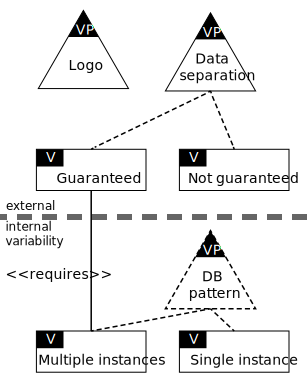
\includegraphics[width=0.48\textwidth]{assets/OVM}
    \caption{Example of a Variability Model in OVM notation}
    \label{fig:ovm}
\end{figure}

In OVM, the \textit{variation points} are the key items. One variation point has multiple \textit{variants} that are either optional or mandatory. Relations between VP's exist that define whether some variant is mutual exclusive with some other variant or whether some variant requires an other variant. Relations are drawn as lines between VP's. An example can be seen in figure \ref{fig:ovm}.

% \subsection{Developing with variability in mind}
% Efficient customization of multi-tenant Software-as-a-Service applications with service lines
% by Stefan Walravena, Dimitri Van Landuyta, Eddy Truyena, Koen Handekynb, Wouter Joosena

\subsection{Variability Realization Techniques}
Jansen et al.~\cite{jansen2010customization} note that while lot of research has been done on variability modeling, there is lack of research on techniques needed to implement variability. They identify five realization techniques of two types of customization, being \textit{Model View Controller (MVC) customization} and \textit{system customization}:
\begin{itemize}
\item \textbf{Model changes} allow tenants to fit the application to their domain. Model changes include changing entity attributes, adding entities and entity-relationships. Some changes require a more abstract application and therefore need to be thought upon earlier in the design process than more simple changes which could easily be added later on.
\item Some of the simpler customizations include \textbf{view changes} as in MVC patterns views don't interact with other components, but instead are the receiving part.
\item There is much freedom in \textbf{controller changes}, ranging from restricting data to one tenant only till fully customized workflows.
\end{itemize}
Large systems build of components delivering services can create variations of a different magnitude, on system level:
\begin{itemize}
\item \textbf{System connector changes} occur when connections to remote services are made variable. Examples include having multiple connectors for printing photos or multiple physical mail delivery providers.
\item With \textbf{system component changes} multiple components deliver the same service and are selected based on configuration.
\end{itemize}

Kabbedijk and Jansen~\cite{kabbedijk2011variability} describe three variability realization techniques they observed in case studies. 
\textbf{Customizable Data Views} are a pattern to store tenant specific representation settings, eg. how tenants want to filter or sort their data. 
Although this technique also requires some table storing data and needs a small controller, it can be seen as mainly a view change as described by Jansen et al. 
Another view change is the \textbf{Module Dependent Menu}-pattern, to create menus that are dependent on the modules associated to a tenant. The last technique they observe is more a controller change. 
\textbf{Pre/Post Update Hooks} is a pattern to execute pieces of code before or after certain events happen in the application. 
This allows for tenants to enable or disable modules that check data or automate certain tasks.

A common way to implement controller changes or system component changes is the variation technique \textbf{dependency injection (DI)} where one of the (possibly many) classes that implement the same interface are injected by a provider. 
Walraven, Truyen and Joosen~\cite{walraven2011middleware} created a middleware layer that uses a existing DI framework, compatible with Google App Engine, named Guice. An issue with Guice, that did not allow per-request switching of implementations was quickly solved by adding a small abstraction layer, making Guice usable in a multi-tenant environment.
Side note: their case study also shows that GAE leverages the effort of separating tenant data a lot by providing the so-called Namespaces API. By linking each tenant to an unique namespace all data in that namespace is only accessible by a that specific tenant.

One of the conclusions of Walraven et al. is that Aspect Oriented Software Development (AOSD) looks promising as an alternative to DI for more complex customizations, such as features that have to be combined.
They go further on this lead in Truyen et al.~\cite{truyen2012context} and introduce \textbf{Context Oriented Programming (COP)}, a form of AOSD to implement what can be seen as controller changes. 
In COP layers are added to the code that override certain behavior when this layer is activated for a specific tenant. 
In DI, for each variation point only one variation can be injected at a time, so no two 'modules' providing the same functionality can interact or extend each other, while in COP those implementations can work together, because the overriding methods can still call the original method allowing them to modify the output or implement a filter. 
Multiple layers can be active at once, doing their work in a predefined order. 
% MAYBE-TODO: this paragraph could be more elaborate

\subsection{Research Agenda for Variability}
% svahnberg2005taxonomy
% sun2008software: no interesting future work proposed

% mietzner2008defining: automization, no further interesting future work proposed
Mietzner et al.~\cite{mietzner2008defining} want to make variability easier to manage for SaaS providers and created so called \textit{solutions} that define which variants should be bound. In the future it could be investigated how deployment scripts could be derived from those solutions.

Mietzner et al.~\cite{mietzner2009variability} describe a cost model for SaaS applications to compare the cost of multi tenant aware versus non-multi-tenant aware applications. They do not however relate this cost model to their variability model. This is interesting for future research as a SaaS provider can then determine the cost of creating, maintaining and managing a variant. The provider could then decide if it economically makes more sense to keep a variant or to remove it.

% jansen2010customization nothing in this paper thats not in kabbedijk2011variability

While Kabbedijk and Jansen~\cite{kabbedijk2011variability} have determined some Variability Realization Techniques, but note that more VRTs could be identified and should be tested on effectiveness, maintainability, scalability and performance.

Truyen et al.~\cite{truyen2012context} found that COP was useful as a VRT but ContextJ lacked support for asynchronous request because context is not shared to new threads. Research could be done to see if it is possible to bridge this gap to make COP more usable as more and more applications are using asynchronous functionality.

Furthermore they found that Google App Engine scales well automatically, but does not support any kind of performance isolation or can guarantee performance to any specific tenant more than an other tenant. More research can be done on this subject and maybe Google and other PaaS providers will then implement this functionality and enable SaaS providers using their platform to sell Quality of Service guarantees.

Another open issue that Truyen et al. identify is maintaining global state consistency when doing updates. The tenants that don't use any of the updated functionality should not experience any interruptions. When SLAs are sold this consistency and uninterrupted service should be provable.

% schroeter2012towards

\section{Conclusion}
\label{sec:conclusion}
In this paper we surveyed the current state of multi-tenancy research.
We have identified several topics for further research on the subjects of security, scalability, quality of service and variability.

Multi-tenancy can be divided in three levels: a shared application with a separated database, a shared application with a shared database (separate schema) and a shared application with a shared schema~\cite{bezemer2010multi}. The latter is considered pure or native multi-tenancy~\cite{bezemer2010multi,lin2009feedback,aulbach2009comparison}.

The relationship between multi-tenancy and the \ac{SaaS} domain is considered close~\cite{dillon2010cloud}, or even stronger: multi-tenancy is a characteristic of the \ac{SaaS} domain~\cite{tsai2010towards}. Additionally, the challenges of cloud services overlap with the challenges of multi-tenancy~\cite{dillon2010cloud,krebs2012architecture}.

In Section~\ref{sec:security} on security, an overview has been provided of the new security concerns and their solutions introduced in multi-tenancy, including data localization, data storage and authentication and authorization. We showed that there is a thin line between security issues caused by multi-tenancy and security issues caused by the general cloud technologies. Multi-tenancy is a high-level concept, relying on a multitude of other technologies, which thereby inherits traditional security issues.  

In Section~\ref{sec:scalability} on scalability, research on estimating resource consumption per tenant and using these estimations to place tenants within the existing infrastructure was discussed. In addition to that an overview of data layer specific scalability research was presented.

\ac{QoS} research was surveyed separately from scalability. Three techniques that use a form of per tenant request limiting for separating tenants were discussed.

On the subject of variability, most research is done on modeling variations and describing techniques to build variants. We provided an overview of the levels of variability (e.g. external variability, visible to the customer; and internal variability, invisible to the customer), three modeling techniques (Feature modeling, Decision modeling and Orthogonal Variability modeling) and the various variation techniques.

\subsection{Research Agenda}
\label{sec:ra}
Throughout the paper we identified several research opportunities. Below we list the most prominent opportunities. Some of the opportunities described earlier fit into a certain category. These opportunities have been merged.
\begin{itemize}

\item \textbf{Automation}. 
To exploit economies of scale, providers of multi-tenant applications want to attract as many tenants and users as possible. 
However, managing all these tenants and their configurations takes a lot of time without the proper tools. 
Research has been done on creating wizards for tenants~\cite{mietzner2008generation,mietzner2008defining}, but this field is not completely covered yet and additionally, automatic deployment of the outcome of these wizards can be investigated (Section~\ref{sec:var_agenda}).
\item \textbf{Guarantees}. 
In all aspects of multi-tenancy new problems arise. 
The solutions proposed for these problems need to be provable, for multi-tenancy to be usable in high availability or business critical applications. 
Open research opportunities lie in state consistency while updating the platform (Section~\ref{sec:var_agenda}), proving data isolation between tenants (Section~\ref{sec:security_agenda}), providing performance isolation and minimal performance (Section~\ref{sec:qos_agenda}).
\item \textbf{Effective security}.
Although security measures have been proposed to secure multi-tenant systems, research should be dedicated to finding a effective balance between security and performance. Traditional and new security mechanisms should be redesigned to increase their effectiveness in multi-tenancy environments (Section~\ref{sec:security_agenda}).
\item \textbf{Tenant aware components}.
In scalability and \ac{QoS} research, tools like tenant aware load balancers and tenant aware databases are used or proposed (Section~\ref{sec:scal_mta} and \ref{sec:tenant_aware}).
The benefits of such tools in a multi-tenant environment have already been proven.
The proposed multi-tenant aware database is still incomplete as it lacks tenant aware administration tooling and more work on the storage model is needed. 
Also, the approaches used for making load balancers multi-tenant aware, need to be validated further.

%\item \highlight{Voeg hier je belangrijkste punten toe}  en probeer te kijken of het niet overlapt met andere punten en zo ja: voeg samen.
\end{itemize}

\section{Acknowledgements}
This literature survey was done in the context of the TI3700 course on the Delft University of Technology. We thank Cor-Paul Bezemer, as our first reviewer, for his helpful comments to improve this paper.

\bibliographystyle{plain}
\bibliography{ref}

\end{document}
